% ------------------------------------------------------------
% ------------------------------------------------------------
  
% Insert the common KETCube AppNote Defines

% ------------------------------------------------------------
% ------------------------------------------------------------

\documentclass[twoside,a4paper,usenames,dvipsnames]{refart}
\usepackage[utf8x]{inputenc}
%\usepackage[czech]{babel}
\usepackage[pdftex]{graphicx}
\graphicspath{{resources/images/}}
\usepackage{caption}% for \captionof
\usepackage{mwe}% contains example-image

% Definition of shortcuts for authornames
%  Sort alphabetically by surname

\newcommand{\JB}{Jan Bělohoubek}
\newcommand{\JC}{Jiří Čengery}
\newcommand{\JF}{Jaroslav Freisleben}
\newcommand{\PK}{Petr Kašpar}
\newcommand{\MU}{Matin Úbl}
\newcommand{\KV}{Kryštof Vaněk}
\newcommand{\JZ}{Jan Záruba}


\usepackage[owncaptions]{vhistory}
\usepackage{hyperref}
%\usepackage[superscript,biblabel]{cite}
\usepackage{multirow}
\usepackage{wrapfig}
\usepackage{float}
\usepackage{siunitx}
\usepackage[table, x11names]{xcolor}
\usepackage{fancyvrb}
\usepackage{fontawesome}
\usepackage[many]{tcolorbox}
\usepackage{listings}
\usepackage{tikz}
\usetikzlibrary{shapes,positioning}
\usepackage{verbatimbox}

\usepackage{array, booktabs, boldline} %
\usepackage{mathtools}
\usepackage[normalem]{ulem}

\usepackage[T1]{fontenc}% Needed for \textquotedbl
\DeclareSIUnit[number-unit-product = {}]{\inchQ}{\textquotedbl}

\newsavebox{\tempbox}
\newlength{\tempheight}

\newcommand\ToDo[1]{\textcolor{red}{ToDo: #1}}

% --- Boxed Enviroments

\newcommand\docNote[1]{
\par
\addvspace{0.5cm}
\subsubsection*{~\hspace{0.2cm}\textcolor{gray}{\Huge \faCommentingO\,}}
\vspace{-1.5cm}
\begin{tcolorbox}[breakable,colback=white,colframe=gray,width=\dimexpr\textwidth+32mm\relax,enlarge left by=-32mm, title = Note]
\it \small #1
\end{tcolorbox}
}

\newcommand\docWarn[1]{
\par
\addvspace{0.5cm}
\subsubsection*{~\hspace{0.2cm}\textcolor{gray}{\Huge \faWarning\,}}
\vspace{-1.5cm}
\begin{tcolorbox}[breakable,colback=white,colframe=gray,width=\dimexpr\textwidth+32mm\relax,enlarge left by=-32mm, title = Warning]
\it #1
\end{tcolorbox}
}

\newcommand\docExample[1]{
\par
\addvspace{0.5cm}
\subsubsection*{~\hspace{0.2cm}\textcolor{gray}{\Huge \faCogs\,}}
\vspace{-1.5cm}
\begin{tcolorbox}[breakable,colback=white,colframe=gray,width=\dimexpr\textwidth+32mm\relax,enlarge left by=-32mm, title = Example]
#1
\end{tcolorbox}
}

\newenvironment{docCodeExample}
{
\par
\addvspace{0.5cm}
\subsubsection*{~\hspace{0.2cm}\textcolor{gray}{\Huge \faCogs\,}}
\vspace{-1.5cm}
\begin{tcolorbox}[breakable,colback=white,colframe=gray,width=\dimexpr\textwidth+32mm\relax,enlarge left by=-32mm, title = Example]
}
{
\end{tcolorbox}
}

\newenvironment{docCodeExampleTitled}[1]
{
\par
\addvspace{0.5cm}
\subsubsection*{~\hspace{0.2cm}\textcolor{gray}{\Huge \faCogs\,}}
\vspace{-1.5cm}
\begin{tcolorbox}[breakable,colback=white,colframe=gray,width=\dimexpr\textwidth+32mm\relax,enlarge left by=-32mm, title = Example: #1]
}
{
\end{tcolorbox}
}

% --- Filesystem Names 
\newcommand\docPath[1]{{\tt #1}}
\newcommand\docFileName[1]{{\tt #1}}

% --- Source Code Names 
\newcommand\docVarName[1]{{\tt #1}}
\newcommand\docFnName[1]{{\tt #1}}
\newcommand\docTypeName[1]{{\tt #1}}

% --- KETCube Terms
\newcommand\docKCModName[1]{{\it #1} module}
\newcommand\docKCCmdInline[1]{\colorbox{gray!30}{\tt #1}}
\newcommand\docKCCmd[1]{{\tt > #1}}

% --- NICE sections
\newcommand\niceSubSection[2]{
\subsection*{~\hspace{0.2cm}{\Huge #1}\\[-0.6cm]\phantom{x}~\hspace{1cm}~#2}
\vspace{-0.7cm}
}

%skryt barevny obdelnik kolem odkazu
\hypersetup{
    colorlinks=false,
    pdfborder={0 0 0},
}

% vhistory
\renewcommand{\vhhistoryname}{Revision History}
\renewcommand{\vhchangename}{Note}
\renewcommand{\vhversionname}{Revision}
\renewcommand{\vhdatename}{Date}
\renewcommand{\vhauthorname}{Author}
\renewcommand \vhAuthorColWidth{0.8\hsize}
\renewcommand \vhChangeColWidth{1.2\hsize}

\DeclareRobustCommand{\UWBLogo}{%
   \begin{wrapfigure}{l}{2.1cm}
    \vspace{-1.35cm}
    \includegraphics[width=2cm]{ZCU_logo.pdf}
   \end{wrapfigure}
}


% declare the path(s) where your graphic files are
% extract presenattion number to create include path for images
\ExplSyntaxOn
% Save a copy of \jobname
\tl_set:NV \NUMBER \c_sys_jobname_str
\regex_replace_once:nnN { [A-Za-z]*_[A-Za-z]*_ } { } \NUMBER
\ExplSyntaxOff

% declare the path(s) where your graphic files are
%\graphicspath{{resources/images/}{resources/appNotes/001/images/}}
\graphicspath{{resources/images/}{resources/appNotes/\NUMBER/images/}}
\graphicspath{{resources/images/}{resources/appNotes/003/images/}}

\pdfinfo
{
  /Title       (The KETCube Project AppNote)
  /Creator     (LaTeX)
  /Author      (The SmartCAMPUS Team)
}




\title{\UWBLogo KETCube AppNote 005:\\ KETCube Terminal (\vhCurrentVersion)}

\author{Author: \vhListAllAuthorsLongWithAbbrev}
\date{Version \vhCurrentVersion\ from \vhCurrentDate}

% ------------------------------------------------------------
% ------------------------------------------------------------
  
% Insert the common KETCube AppNote Head

% ------------------------------------------------------------
% ------------------------------------------------------------

\begin{document}
\pagenumbering{roman} 

\titlepage
\maketitle

% ------------------------------------------------------------
% ------------------------------------------------------------
  
% BEGIN of the KETCube appNote Content

% ------------------------------------------------------------
% ------------------------------------------------------------


% ------------------------------------------------------------
% ------------------------------------------------------------
  
% BEGIN of the KETCube appNote Content

% ------------------------------------------------------------
% ------------------------------------------------------------

\section*{About this Document}
{\it KETCube} \cite{ZCU:KETCube:05-2018} is the prototyping and demo platform developed at the Department of Materials and Technology (KET), University of West Bohemia in Pilsen. 


This document describes KETCube Terminal. 

\setcounter{tocdepth}{2}
\tableofcontents
\clearpage

\listoffigures
\listoftables
\begin{versionhistory}
  \vhEntry{0.2.0*}{5.1.2021}{JB}{Initial version}
\end{versionhistory}
% history table ... do not number
\setcounter{table}{0}

\clearpage 
\pagenumbering{arabic} 
\pagestyle{headings} 

\clearpage 
\section{KETCube Terminal Interface}
When programmed by the supplied software stack, the KETCube serial interface called {\it KETCube Terminal} is available on USART1 (IO1 and IO2) -- see Figure \ref{fig:terminal:putty}. KETCube Terminal allows to configure KETCube platform, KETCube modules (e.g. HDC1080, batVoltage, LoRa ...) and module parameters (e.g. devEUI, appKEY, ... for LoRa module). The KETCube terminal is case-sensitive.

The interface physical settings are as follows:

\begin{itemize}
  \item Tx PIN: PA9
  \item Rx PIN: PA10
  \item Speed: 9600 bps
  \item Data bits: 8
  \item Stop bits: 1
  \item Parity: No
  \item HW Flow control: No
  \item End-of-line: CR+LF or LF
\end{itemize}

\clearpage
\section{KETCube Command Set}
The Terminal commands follow the hierarchical tree arrangement. The basic help including root commands is printed after device reset. The command \docKCCmdInline{help} can be used anytime to display root commands.

Inline help is displayed when \docKCCmdInline{[TAB]} key is pushed (e.g. write \docKCCmdInline{s[TAB]} and all commands with leading \docKCCmdInline{s} will be printed -- these are: \docKCCmdInline{set}, \docKCCmdInline{show}, \docKCCmdInline{setr} and \docKCCmdInline{showr}). Inline help is usefull especially for commands hidden deeply in the tree structure.

To display list of modules use \docKCCmdInline{list} command. Commands \docKCCmdInline{enable}/\docKCCmdInline{disable} are used to turn ON/OFF KETCube modules (e.g. \docKCCmdInline{enable HDCX080}). 

The \docKCCmdInline{enable} command can be additionally used to set the severity level -- the second (optional) parameter of the command sets the module {\it severity level}. The {\it severity level} defines the amount of information provided by the specified module to the Terminal. Use the following command to enable {\it HDCX080}, while setting the {\it severity level} to {\it INFO}: \docKCCmdInline{enable HDCX080 2}.

Commands \docKCCmdInline{show}/\docKCCmdInline{set} are used to show/set KETCube settings (e.g. \docKCCmdInline{show LoRa devEUI}). Parameters are saved into on-chip EEPROM and take effect after the device reset (command \docKCCmdInline{reload} or power-cycle).

Commands \docKCCmdInline{showr}/\docKCCmdInline{setr} are used to show/set KETCube running settings (e.g. \docKCCmdInline{showr LoRa devAddr}). Parameters are saved into RAM and take effect immediately.

The commands \docKCCmdInline{show(r)}/\docKCCmdInline{set(r)} are used to show/set KETCube (module) settings. The commands are organized in a tree-like manner: the \docKCCmdInline{show(r)}/\docKCCmdInline{set(r)} command is the root command, it is followed by the module name (or the keyword \docKCCmdInline{core} for the KETCube platform settings) and by the module (or core) parameter, which is to be set/show. 

KETCube Terminal provides also the command history, which is available through {\tt <} and {\tt >} keys.

\marginlabel{\captionof{figure}{KETCube Terminal in Putty}\label{fig:terminal:putty}}
\raisebox{-\height}{\includegraphics[width=0.5\paperwidth]{ketCube_terminal_putty.png}}

\clearpage
\section{KETCube Modules}\label{sec:modules}
KETCube is a modular platform, where number of modules is included in the platform release. Any module can be individually enabled or disabled based on user needs and extension boards connected to the KETCube {\it Main Board}. For details, please refer to the KETCube Datasheet \cite{ZCU:KETCube:05-2018} or appNote 006 \cite{ZCU:KETCubeAppNote006:09-2019}, where module parameters are described.

To display list of available modules, open the KETCube Terminal and use \docKCCmdInline{list} command. Commands \docKCCmdInline{enable}/\docKCCmdInline{disable} are used to turn ON/OFF modules (e.g. \docKCCmdInline{enable HDCX080}). When module is enabled, it starts to perform defined operation (e.g. measure RH and Temperature).

Debug messages are useful when device is initially configured or in case, that unexpected behavior occurred.

Debug messages are printed to serial terminal interface. They can be configured on the per-module basis by setting the {\it severity level} to the selected module or to the KETCube core.

Four severity levels are defined:
\begin{itemize}
  \item[0 --] NONE -- no messages enabled
  \item[1 --] ERROR -- only error messages enabled (default severity)
  \item[2 --] INFO -- error and informational messages enabled
  \item[3 --] DEBUG -- previous message groups and debug information are enabled
\end{itemize}

The second (optional) parameter of the \docKCCmdInline{enable} command is used to configure the {\it severity level} of the selected module (e.g. \docKCCmdInline{enable HDC1080 3} enables debug messages for HDCX080 module). The default  {\it severity level} is {\it ERROR}. The command \docKCCmdInline{set core severity} is used to configure \docKCCmdInline{severity level} of the KETCube core and command \docKCCmdInline{set driver severity} is used to configure {\it severity level} of the KETCube low-level drivers.

\docNote{Debug messages may cause a situation, where it may be difficult to write commands (terminal echo is foggy due to lot of debug messages produced by KETCube)}.

\clearpage 
\section{KETCube Remote Terminal}
When programmed by the supplied software stack, the {\it KETCube Remote Terminal} feature is available in KETCube. The {\it KETCube Remote Terminal} allows to execute KETCube commands remotely. Only the LoRaWAN network is currently supported (loraserver.io with MQTT interface was the test platform). Note, that the remote execution is enabled for ``safe'' commands only.

To control KETCube over LoRaWAN, you need a well-configured KETCube connected to the LoRaWAN network (reliable downlink is required). The {\it KETCube Remote Terminal} tool\footnote{\url{https://github.com/SmartCAMPUSZCU/KETCube-remote-terminal}} is used to configure KETCube remotely.

The {\it KETCube Remote Terminal} uses a configuration file \docFileName{config.ini}, where connection settings to the LoRaWAN application server are defined (e.g. server address, timeout, Rx and Tx topics). After writing settings into \docFileName{config.ini}, the {\it KETCube Remote Terminal} tool can be executed:

\begin{Verbatim}[frame=single, fontsize=\small]
$ ./ketcube-remote-terminal
\end{Verbatim}

The tool accepts KETCube commands in the same form as the KETCube serial Terminal. Note, that the response to the command may be delayed significantly, depending on the KETCube and the network settings and the link reliability. 

Due to increased latency given by network communication, {\it KETCube Remote Terminal} tool implements the {\it batch mode} allowing the command sequence execution:

\begin{Verbatim}[frame=single, fontsize=\small]
!batch
enable ADC
disable TxDisplay
set core basePeriod 360000
!commit
reload
\end{Verbatim}


\clearpage 
\section{KETCube Remote Terminal Protocol}

The remote terminal protocol is an application protocol built on top of any supported undelying general-purpose application protocol like MQTT. Thus, it is designed to contain only application-level logic. Each packet starts with a 16-bit header. Its structure is as follows.

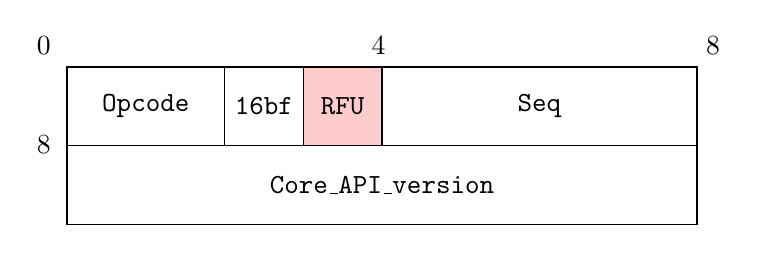
\begin{tikzpicture}
 \node[draw,anchor=north west,yshift=1.5cm,fill=white,minimum height=1cm,minimum width = 2cm,xshift=0cm,]{\texttt{Opcode}};
 \node[draw,anchor=north west,yshift=1.5cm,fill=white,minimum height=1cm,minimum width = 1cm,xshift=2cm]{\texttt{16bf}};
 \node[draw,anchor=north west,yshift=1.5cm,fill=red!20,minimum height=1cm,minimum width = 1cm,xshift=3cm]{\texttt{RFU}};
 \node[draw,anchor=north west,yshift=1.5cm,fill=white,minimum height=1cm,minimum width = 4cm,xshift=4cm]{\texttt{Seq}};
 \node[draw,anchor=north west,yshift=0.5cm,fill=white,minimum height=1cm,minimum width = 8cm,xshift=0cm]{\texttt{Core\_API\_version}};
 \node[anchor=north west,yshift=2.0cm,xshift=-0.5cm,fill=white] {0};
 \node[anchor=north west,yshift=2.0cm,xshift=+3.75cm,fill=white] {4};
 \node[anchor=north west,yshift=2.0cm,xshift=+8.0cm,fill=white] {8};
 
 \node[anchor=north west,yshift=0.75cm,xshift=-0.5cm,fill=white] {8};
\end{tikzpicture}

\begin{itemize}
	\item \texttt{Opcode} - [2b] operation code
		\begin{itemize}
			\item \texttt{CMD} (value 0) - the packet comprises a single command
			\item \texttt{BATCH} (value 1) - the packet comprises a batch of commands
		\end{itemize}
	\item \texttt{16bf} - [1b] 16bit module ID flag
		\begin{itemize}
			\item if set, all module IDs present in payload are encoded as 16bit unsigned integers
			\item otherwise, 8bit unsigned integer encoding is used
			\item 16bit IDs can be used anytime; 8bit IDs save payload, but they are only allowed when all IDs in a single command are lower than 256 (typically for \texttt{core} command)
		\end{itemize}
	\item \texttt{RFU} - [1b] Reserved for Future Use
	\item \texttt{Seq} - [4b] sequence number
		\begin{itemize}
			\item command sequence number for pairing requests with responses
		\end{itemize}
	\item \texttt{Core\_API\_version} - [8b] version of core API
		\begin{itemize}
			\item core API versions should match on both sides
			\item mismatch may lead to command rejection
			\item the core API version for KETCube v0.2 is \texttt{0x04}
		\end{itemize}
\end{itemize}

The payload structure differs by used opcode. All values are encoded as little-endian.

\subsection{Single command packet payload}

A single command packet payload structure is as follows.

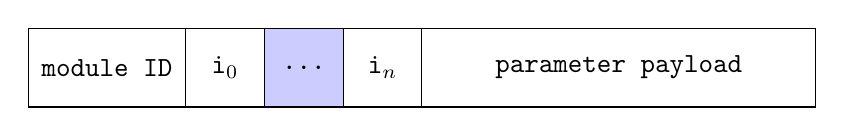
\begin{tikzpicture}
 \node[draw,anchor=north west,yshift=1.5cm,fill=white,minimum height=1cm,minimum width = 2cm,xshift=0cm,]{\texttt{module ID}};
 \node[draw,anchor=north west,yshift=1.5cm,fill=white,minimum height=1cm,minimum width = 1cm,xshift=2cm]{\texttt{i$_0$}};
 \node[draw,anchor=north west,yshift=1.5cm,fill=blue!20,minimum height=1cm,minimum width = 1cm,xshift=3cm]{\texttt{\dots}};
 \node[draw,anchor=north west,yshift=1.5cm,fill=white,minimum height=1cm,minimum width = 1cm,xshift=4cm]{\texttt{i$_n$}};
 \node[draw,anchor=north west,yshift=1.5cm,fill=white,minimum height=1cm,minimum width = 5cm,xshift=5cm]{\texttt{parameter payload}};
\end{tikzpicture}

\begin{itemize}
	\item \texttt{module ID} - [8b or 16b] ID of module from global enumeration
		\begin{itemize}
			\item marks that the command targets a specified module ID
			\item generic or non-targetted commands is assumed to target the core API (\texttt{KETCUBE\_MODULEID\_CORE\_API})
		\end{itemize}
	\item \texttt{command tree path} - [at least 8b] an array of 1-byte indexes to terminal command tree
		\begin{itemize}
			\item each field represents an index in the command (sub-)tree
			\item parsing is ended implicitly when a leaf (specific command) is reached
			\item module index in the \texttt{set}/\texttt{setr} and \texttt{show}/\texttt{showr} tree is skipped, as the moduleID specifies the module
		\end{itemize}
	\item \texttt{parameter payload} - [variable length] serialized parameters of a given command
		\begin{itemize}
			\item if the command does not require any parameters, this field is missing
			\item parameters are serialized by custom rules mentioned below
		\end{itemize}
\end{itemize}

The command tree path is retrieved by traversing the terminal command tree. If a generic command is addressed, module ID is ignored. Parsing may go through 3 phases:

\begin{itemize}
	\item \texttt{root} - looking for the root command subtree (always a generic entry)
	\item \texttt{module} - looking for a module in given subtree - this avoids conflicts between same base versions with different module set selected during compilation; this level is thus not identified by index to an array, but rather by module ID itself
	\item \texttt{subtree} - looking for a specific subtree or command
\end{itemize}

\docExample{
Command with 8bit module ID and 4byte payload encoding:
\vspace{0.4cm}

\resizebox{\textwidth}{!}{
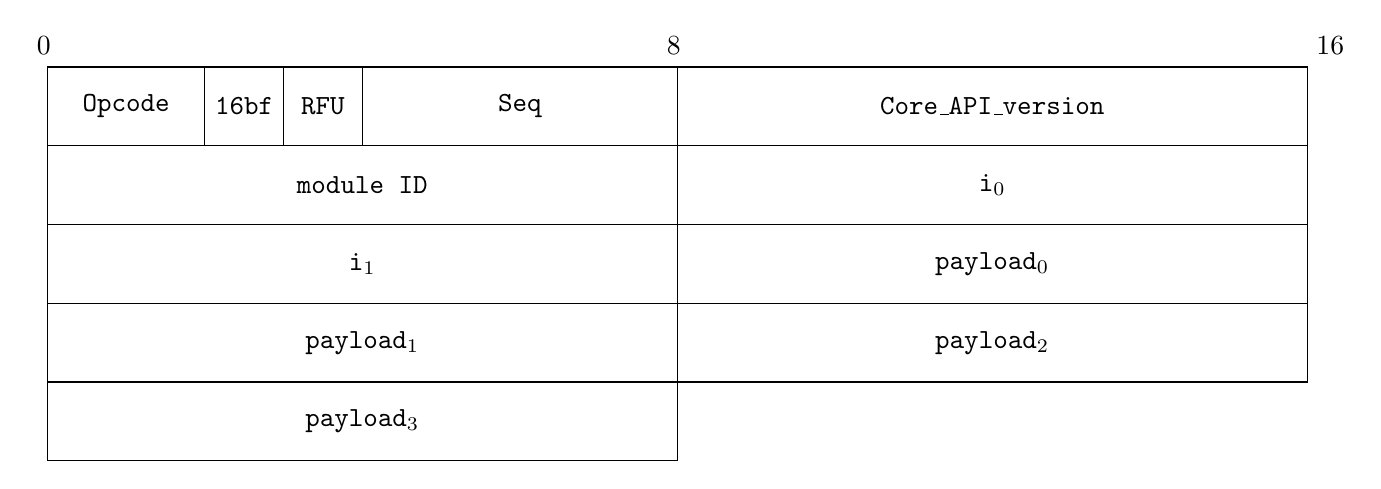
\begin{tikzpicture}
 \node[draw,anchor=north west,yshift=4.5cm,fill=white,minimum height=1cm,minimum width = 2cm,xshift=0cm,]{\texttt{Opcode}};
 \node[draw,anchor=north west,yshift=4.5cm,fill=white,minimum height=1cm,minimum width = 1cm,xshift=2cm]{\texttt{16bf}};
 \node[draw,anchor=north west,yshift=4.5cm,fill=white,minimum height=1cm,minimum width = 1cm,xshift=3cm]{\texttt{RFU}};
 \node[draw,anchor=north west,yshift=4.5cm,fill=white,minimum height=1cm,minimum width = 4cm,xshift=4cm]{\texttt{Seq}};
 \node[draw,anchor=north west,yshift=4.5cm,fill=white,minimum height=1cm,minimum width = 8cm,xshift=8cm]{\texttt{Core\_API\_version}};
 \node[draw,anchor=north west,yshift=3.5cm,fill=white,minimum height=1cm,minimum width = 8cm,xshift=0cm]{\texttt{module ID}};
 \node[draw,anchor=north west,yshift=3.5cm,fill=white,minimum height=1cm,minimum width = 8cm,xshift=8cm]{\texttt{i$_0$}};
 \node[draw,anchor=north west,yshift=2.5cm,fill=white,minimum height=1cm,minimum width = 8cm,xshift=0cm]{\texttt{i$_1$}};
 \node[draw,anchor=north west,yshift=2.5cm,fill=white,minimum height=1cm,minimum width = 8cm,xshift=8cm]{\texttt{payload$_0$}};
 \node[draw,anchor=north west,yshift=1.5cm,fill=white,minimum height=1cm,minimum width = 8cm,xshift=0cm]{\texttt{payload$_1$}};
 \node[draw,anchor=north west,yshift=1.5cm,fill=white,minimum height=1cm,minimum width = 8cm,xshift=8cm]{\texttt{payload$_2$}};
 \node[draw,anchor=north west,yshift=0.5cm,fill=white,minimum height=1cm,minimum width = 8cm,xshift=0cm]{\texttt{payload$_3$}};
 
 \node[anchor=north west,yshift=5.0cm,xshift=-0.25cm,fill=white] {0};
 \node[anchor=north west,yshift=5.0cm,xshift=+7.75cm,fill=white] {8};
 \node[anchor=north west,yshift=5.0cm,xshift=+16.0cm,fill=white] {16};
\end{tikzpicture}
}

\vspace{0.5cm}
Command \docKCCmdInline{set core basePeriod 10000} encoding:
\vspace{0.4cm}

\resizebox{\textwidth}{!}{
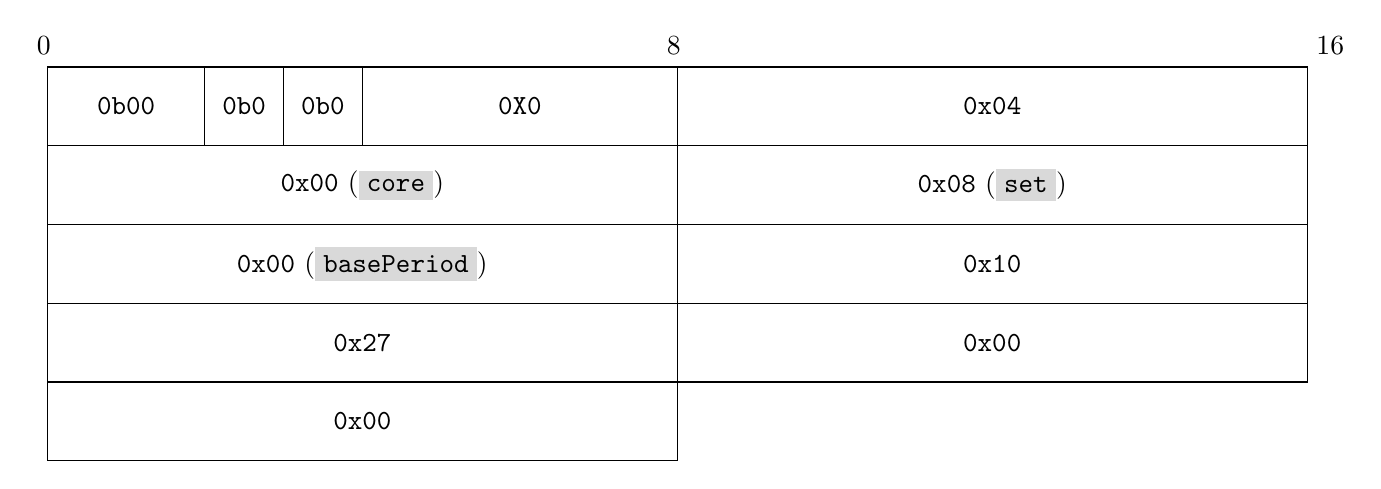
\begin{tikzpicture}
 \node[draw,anchor=north west,yshift=4.5cm,fill=white,minimum height=1cm,minimum width = 2cm,xshift=0cm,]{\texttt{0b00}};
 \node[draw,anchor=north west,yshift=4.5cm,fill=white,minimum height=1cm,minimum width = 1cm,xshift=2cm]{\texttt{0b0}};
 \node[draw,anchor=north west,yshift=4.5cm,fill=white,minimum height=1cm,minimum width = 1cm,xshift=3cm]{\texttt{0b0}};
 \node[draw,anchor=north west,yshift=4.5cm,fill=white,minimum height=1cm,minimum width = 4cm,xshift=4cm]{\texttt{0X0}};
 \node[draw,anchor=north west,yshift=4.5cm,fill=white,minimum height=1cm,minimum width = 8cm,xshift=8cm]{\texttt{0x04}};
 \node[draw,anchor=north west,yshift=3.5cm,fill=white,minimum height=1cm,minimum width = 8cm,xshift=0cm]{\texttt{0x00} (\docKCCmdInline{core})};
 \node[draw,anchor=north west,yshift=3.5cm,fill=white,minimum height=1cm,minimum width = 8cm,xshift=8cm]{\texttt{0x08} (\docKCCmdInline{set})};
 \node[draw,anchor=north west,yshift=2.5cm,fill=white,minimum height=1cm,minimum width = 8cm,xshift=0cm]{\texttt{0x00} (\docKCCmdInline{basePeriod})};
 \node[draw,anchor=north west,yshift=2.5cm,fill=white,minimum height=1cm,minimum width = 8cm,xshift=8cm]{\texttt{0x10}};
 \node[draw,anchor=north west,yshift=1.5cm,fill=white,minimum height=1cm,minimum width = 8cm,xshift=0cm]{\texttt{0x27}};
 \node[draw,anchor=north west,yshift=1.5cm,fill=white,minimum height=1cm,minimum width = 8cm,xshift=8cm]{\texttt{0x00}};
 \node[draw,anchor=north west,yshift=0.5cm,fill=white,minimum height=1cm,minimum width = 8cm,xshift=0cm]{\texttt{0x00}};
 
 \node[anchor=north west,yshift=5.0cm,xshift=-0.25cm,fill=white] {0};
 \node[anchor=north west,yshift=5.0cm,xshift=+7.75cm,fill=white] {8};
 \node[anchor=north west,yshift=5.0cm,xshift=+16.0cm,fill=white] {16};
\end{tikzpicture}
}
}

\clearpage
\subsection{Batch packet payload}

A batch packet payload structure is as follows:

\begin{itemize}
	\item \texttt{length} - [8b] length of the payload
		\begin{itemize}
			\item excludes fixed-size common header and self
		\end{itemize}
	\item \texttt{module ID} - [8b or 16b] module ID, unused for now
		\begin{itemize}
			\item reserved, set to 0 for all batch packets
		\end{itemize}
	\item \texttt{command array} - [variable length] an array of single command packet payloads
\end{itemize}

\docNote{The \textit{16bf} field of the common header is set, if any of commands in the batch addresses a module with 16-bit ID. Thus, this bit affects every command encoded within this batch.}.

\subsection{Parameter encoding rules}

The parameters are encoded in minimalistic fashion due to the fact, that both sides of communication are informed about transfered data types, their limitations and sizes.

\begin{itemize}
	\item \texttt{KETCUBE\_TERMINAL\_PARAMS\_BOOLEAN} - encoded as a one-byte unsigned character, 0 represents \textit{false}, any other value represents \textit{true}
	\item \texttt{KETCUBE\_TERMINAL\_PARAMS\_BYTE} - encoded as a one-byte unsigned character
	\item \texttt{KETCUBE\_TERMINAL\_PARAMS\_MODULEID} - encoded as a pair of 16bit module ID (always 16bit, regardless the \textit{16bf} flag) and a 8bit severity identifier
	\item \texttt{KETCUBE\_TERMINAL\_PARAMS\_INT32} - encoded as a 32-bit signed integer in target machine representation
	\item \texttt{KETCUBE\_TERMINAL\_PARAMS\_UINT32} - encoded as a 32-bit unsigned integer
	\item \texttt{KETCUBE\_TERMINAL\_PARAMS\_STRING} - encoded as a sequence of bytes terminated with zero-character; the array itself has a fixed-size of \texttt{KETCUBE\_TERMINAL\_PARAM\_STR\_MAX\_LENGTH}
	\item \texttt{KETCUBE\_TERMINAL\_PARAMS\_INT32\_PAIR} - encoded as two subsequent 32-bit signed integers in target machine representation
	\item \texttt{KETCUBE\_TERMINAL\_PARAMS\_BYTE\_ARRAY} - encoded as a fixed-length byte array and a 16bit length; the length represents the actual number of bytes used within the given fixed-size array; the array size is \texttt{KETCUBE\_TERMINAL\_PARAM\_BYTE\_ARRAY\_MAX\_LENGTH}
\end{itemize}

All values are encoded as little-endian.

\subsection{Command response}

The response always contains the same header, as the request. To properly pair the request with response, a packet opcode and its sequence number is used. If any of those fields does not match the expected header fields, the response shoult be discarded and an error should be displayed.

Once the response is properly paired with a request, following fields are extracted:

\begin{itemize}
	\item \texttt{error code} - an 8bit unsigned character representing the command evaluation outcome on the remote side
	\item \texttt{output parameter} - a single output parameter decoded by the same rules as an input parameter
\end{itemize}

The response processing procedure is identical for batch packets, except the extraction procedure is repeated for every command issued in given batch.

To properly identify errors, the remote terminal uses an additional values in \texttt{ketCube\_terminal\_command\_errorCode\_t} enumerator. For more information, please, refer to the source code.

\subsection{Flow}

The protocol uses a simple \textit{Stop-and-wait} communication scheme. This means, that the received and sender window has a length of 1 packet, and no other packet should be sent until the last one is acknowledged (i.e.; a response is received and parsed). No other packet flow-control is required, nor supported. Therefore, this protocol completely relies on underlying protocols to ensure data transfer reliability.

Due to increased latency in network communication, and base period set in the ketCube core configuration, the timeout for remote terminal command responses should be set to a reasonably high value. If the timeout value is exceeded during wait, the command is discarded and no response is further anticipated.

  
% ------------------------------------------------------------
% ------------------------------------------------------------
  
% END of the KETCube appNote Content

% ------------------------------------------------------------
% ------------------------------------------------------------



% ------------------------------------------------------------
% ------------------------------------------------------------
  
% Insert the common KETCube appNote Tail

% ------------------------------------------------------------
% ------------------------------------------------------------

% ------------------------------------------------------------
% ------------------------------------------------------------
  
% END of the KETCube appNote Content

% ------------------------------------------------------------
% ------------------------------------------------------------


\clearpage
\bibliographystyle{IEEEtran}
\bibliography{IEEEabrv,resources/sources}

%
% Include this license into all KETCube-related documentation
%
%

\clearpage

~

\vfill

\section*{Important Notice}

\subsection*{Copyright}
\copyright ~2018 University of West Bohemia in Pilsen\\
All rights reserved.

\subsection*{Developed by}
The SmartCAMPUS Team\\
Department of Technologies and Measurement\\
Faculty of Electrical Engineering\\
www.smartcampus.cz/en $\mid$ www.zcu.cz/en

\subsection*{License\footnotemark}
\footnotetext{{\it University of Illinois/NCSA Open Source License} (\url{https://opensource.org/licenses/NCSA}) -- similar to {\it Modified BSD License}}

Permission is hereby granted, free of charge, to any person obtaining a copy of this software and associated documentation files (the “Software”), to deal with the Software without restriction, including without limitation the rights to use, copy, modify, merge, publish, distribute, sublicense, and/or sell copies of the Software, and to permit persons to whom the Software is furnished to do so, subject to the following conditions:

\begin{itemize}
    \item[--] Redistributions of source code must retain the above copyright notice, this list of conditions and the following disclaimers.
    \item[--] Redistributions in binary form must reproduce the above copyright notice, this list of conditions and the following disclaimers in the documentation and/or other materials provided with the distribution.
    \item[--] Neither the names of The SmartCAMPUS Team, Department of Technologies and Measurement and Faculty of Electrical Engineering University of West Bohemia in Pilsen, nor the names of its contributors may be used to endorse or promote products derived from this Software without specific prior written permission. 
\end{itemize}
THE SOFTWARE IS PROVIDED “AS IS”, WITHOUT WARRANTY OF ANY KIND, EXPRESS OR IMPLIED, INCLUDING BUT NOT LIMITED TO THE WARRANTIES OF MERCHANTABILITY, FITNESS FOR A PARTICULAR PURPOSE AND NONINFRINGEMENT. IN NO EVENT SHALL THE CONTRIBUTORS OR COPYRIGHT HOLDERS BE LIABLE FOR ANY CLAIM, DAMAGES OR OTHER LIABILITY, WHETHER IN AN ACTION OF CONTRACT, TORT OR OTHERWISE, ARISING FROM, OUT OF OR IN CONNECTION WITH THE SOFTWARE OR THE USE OR OTHER DEALINGS WITH THE SOFTWARE. 

\end{document}


\end{document}


